%%%%%%%%%%%%%%%%%%%%%%%%%%%%%%%%%%%%%%%%%%%%%%%%%%%%%%%%%%%%%%%%%%%%%%%%%%%%%%%%
%  Global includes and setup
%%%%%%%%%%%%%%%%%%%%%%%%%%%%%%%%%%%%%%%%%%%%%%%%%%%%%%%%%%%%%%%%%%%%%%%%%%%%%%%%

\usepackage{ifthen}

\setlength{\parindent}{0pt}

%TODOv2 make sure 5' arrow lines up with sequence


%%%%%%%%%%%%%%%%%%%%%%%%%%%%%%%%%%%%%%%%%%%%%%%%%%%%%%%%%%%%%%%%%%%%%%%%%%%%%%%%
%  Font and paragraph
%%%%%%%%%%%%%%%%%%%%%%%%%%%%%%%%%%%%%%%%%%%%%%%%%%%%%%%%%%%%%%%%%%%%%%%%%%%%%%%%

\usepackage{scalefnt}
\usepackage{PTSansCaption} 
\usepackage{PTSansNarrow} 
\newcommand*{\narrowfont}{\fontfamily{PTSansNarrow-TLF}\selectfont}
\newcommand*{\widefont}{\fontfamily{PTSansCaption-TLF}\selectfont}
\renewcommand*\familydefault{\sfdefault} %% Only if the base font of the document is to be sans serif
\usepackage[T1]{fontenc}


%%%%%%%%%%%%%%%%%%%%%%%%%%%%%%%%%%%%%%%%%%%%%%%%%%%%%%%%%%%%%%%%%%%%%%%%%%%%%%%%
%  Colours
%%%%%%%%%%%%%%%%%%%%%%%%%%%%%%%%%%%%%%%%%%%%%%%%%%%%%%%%%%%%%%%%%%%%%%%%%%%%%%%%

\usepackage{pdfpages} 

\definecolor{A}{cmyk}{0.82,0.62,0.11,0.00}
\definecolor{U}{cmyk}{0.31,1.00,0.70,0.35}
\definecolor{T}{cmyk}{0.31,1.00,0.70,0.35}
\definecolor{C}{cmyk}{0.07,0.40,0.00,0.00}
\definecolor{G}{cmyk}{0.23,0.00,0.04,0.00}
\definecolor{lightblue}{cmyk}{0.23,0.00,0.04,0.00}
\definecolor{lightgrey}{cmyk}{0.00,0.00,0.00,0.15}
\definecolor{grey}{cmyk}{0.00,0.00,0.00,0.15}
\definecolor{darkgrey}{cmyk}{0.00,0.00,0.00,0.50}
\definecolor{gray}{cmyk}{0.00,0.00,0.00,0.50}
\definecolor{black}{cmyk}{0.00,0.00,0.00,1.00}
\definecolor{white}{cmyk}{0.00,0.00,0.00,0.00}


%%%%%%%%%%%%%%%%%%%%%%%%%%%%%%%%%%%%%%%%%%%%%%%%%%%%%%%%%%%%%%%%%%%%%%%%%%%%%%%%
%  Draw the codon boxes
%%%%%%%%%%%%%%%%%%%%%%%%%%%%%%%%%%%%%%%%%%%%%%%%%%%%%%%%%%%%%%%%%%%%%%%%%%%%%%%%

\usepackage{tikz}
\usetikzlibrary{arrows}
\usetikzlibrary{positioning}

\tikzstyle{base}=[remember picture, inner sep=0pt, outer sep=0pt]
\tikzstyle{card}=[remember picture, inner sep=0pt, outer sep=0pt, overlay]


% with bleed to use on the aa cards

\newsavebox{\A}
\savebox{\A}{%
    
\begin{tikzpicture}[base]
    \widefont \Huge
        \draw [black, fill=A] (0,0) rectangle (1 + 0.4,1);
        \draw [black, fill=black] (1 + 0.4,0) rectangle (2 + 0.4,1);
        \node [,white] at (1.5 + 0.4,0.5) {A};
        \path [use as bounding box] (0,0) rectangle (2 + 0.4,1);
    \end{tikzpicture}
}

\newsavebox{\T}
\savebox{\T}{%
    
\begin{tikzpicture}[base]
    \widefont \Huge
        \draw [black, fill=T] (0,0) rectangle (1 + 0.4,1);
        \draw [black, fill=black] (1 + 0.4,0) rectangle (2 + 0.4,1);
        \node [,white] at (1.5 + 0.4,0.5) {T};
        \path [use as bounding box] (0,0) rectangle (2 + 0.4,1);
    \end{tikzpicture}
}

\newsavebox{\U}
\savebox{\U}{%
    
\begin{tikzpicture}[base]
    \widefont \Huge
        \draw [black, fill=U] (0,0) rectangle (1 + 0.4,1);
        \draw [black, fill=black] (1 + 0.4,0) rectangle (2 + 0.4,1);
        \node [,white] at (1.5 + 0.4,0.5) {U};
        \path [use as bounding box] (0,0) rectangle (2 + 0.4,1);
    \end{tikzpicture}
}

\newsavebox{\C}
\savebox{\C}{%
    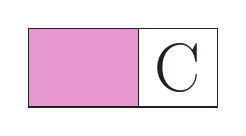
\begin{tikzpicture}[base]
    \widefont \Huge
        \draw [black, fill=C] (0,0) rectangle (1 + 0.4,1);
        \draw [black, fill=white] (1 + 0.4,0) rectangle (2 + 0.4,1);
        \node [,black] at (1.5 + 0.4,0.5) {C};
        \path [use as bounding box] (0,0) rectangle (2 + 0.4,1);
    \end{tikzpicture}
}

\newsavebox{\G}
\savebox{\G}{%
    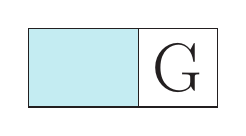
\begin{tikzpicture}[base]
    \widefont \Huge
        \draw [black, fill=G] (0,0) rectangle (1 + 0.4,1);
        \draw [black, fill=white] (1 + 0.4,0) rectangle (2 + 0.4,1);
        \node [,black] at (1.5 + 0.4,0.5) {G};
        \path [use as bounding box] (0,0) rectangle (2 + 0.4,1);
    \end{tikzpicture}
}

\newsavebox{\R}
\savebox{\R}{%
    
\begin{tikzpicture}[base]
    \widefont \Huge
        \draw [black, fill=G] (0,0) rectangle (1 + 0.4, 0.5);
        \draw [black, fill=A] (0,0.5) rectangle (1 + 0.4, 1);
        \draw [black, fill=lightgrey] (1 + 0.4,0) rectangle (2 + 0.4, 1);
        \node [,darkgrey] at (1.5 + 0.4,0.5) {R};
        \path [use as bounding box] (0,0) rectangle (2 + 0.4,1);
    \end{tikzpicture}
}

\newsavebox{\Y}
\savebox{\Y}{%
    
\begin{tikzpicture}[base]
    \widefont \Huge
        \draw [black, fill=C] (0,0) rectangle (1 + 0.4, 0.5);
        \draw [black, fill=U] (0,0.5) rectangle (1 + 0.4, 1);
        \draw [black, fill=lightgrey] (1 + 0.4,0) rectangle (2 + 0.4, 1);
        \node [,darkgrey] at (1.5 + 0.4,0.5) {Y};
        \path [use as bounding box] (0,0) rectangle (2 + 0.4,1);
    \end{tikzpicture}
}

\newsavebox{\HH}
\savebox{\HH}{%
    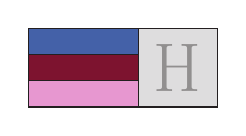
\begin{tikzpicture}[base]
    \widefont \Huge
        \draw [black, fill=C] (0,0) rectangle (1 + 0.4, 0.3333);
        \draw [black, fill=U] (0,0.3333) rectangle (1 + 0.4, 0.6666);
        \draw [black, fill=A] (0,0.6666) rectangle (1 + 0.4, 1);
        \draw [black, fill=lightgrey] (1 + 0.4,0) rectangle (2 + 0.4, 1);
        \node [,darkgrey] at (1.5 + 0.4,0.5) {H};
        \path [use as bounding box] (0,0) rectangle (2 + 0.4,1);
    \end{tikzpicture}
}

\newsavebox{\B}
\savebox{\B}{%
    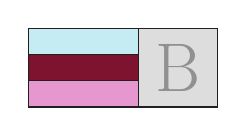
\begin{tikzpicture}[base]
    \widefont \Huge
        \draw [black, fill=C] (0,0) rectangle (1 + 0.4, 0.3333);
        \draw [black, fill=U] (0,0.3333) rectangle (1 + 0.4, 0.6666);
        \draw [black, fill=G] (0,0.6666) rectangle (1 + 0.4, 1);
        \draw [black, fill=lightgrey] (1 + 0.4,0) rectangle (2 + 0.4, 1);
        \node [,darkgrey] at (1.5 + 0.4,0.5) {B};
        \path [use as bounding box] (0,0) rectangle (2 + 0.4,1);
    \end{tikzpicture}
}

\newsavebox{\V}
\savebox{\V}{%
    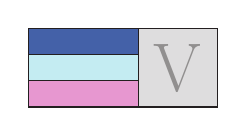
\begin{tikzpicture}[base]
    \widefont \Huge
        \draw [black, fill=C] (0,0) rectangle (1 + 0.4, 0.3333);
        \draw [black, fill=G] (0,0.3333) rectangle (1 + 0.4, 0.6666);
        \draw [black, fill=A] (0,0.6666) rectangle (1 + 0.4, 1);
        \draw [black, fill=lightgrey] (1 + 0.4,0) rectangle (2 + 0.4, 1);
        \node [,darkgrey] at (1.5 + 0.4,0.5) {V};
        \path [use as bounding box] (0,0) rectangle (2 + 0.4,1);
    \end{tikzpicture}
}

\newsavebox{\D}
\savebox{\D}{
    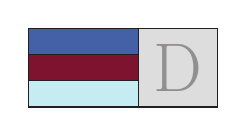
\begin{tikzpicture}[base]
    \widefont \Huge
        \draw [black, fill=G] (0,0) rectangle (1 + 0.4, 0.3333);
        \draw [black, fill=U] (0,0.3333) rectangle (1 + 0.4, 0.6666);
        \draw [black, fill=A] (0,0.6666) rectangle (1 + 0.4, 1);
        \draw [black, fill=lightgrey] (1 + 0.4,0) rectangle (2 + 0.4, 1);
        \node [,darkgrey] at (1.5 + 0.4,0.5) {D};
        \path [use as bounding box] (0,0) rectangle (2 + 0.4,1);
    \end{tikzpicture}
}

\newsavebox{\W}
\savebox{\W}{%
    
\begin{tikzpicture}[base]
    \widefont \Huge
        \draw [black, fill=U] (0,0) rectangle (1 + 0.4, 0.5);
        \draw [black, fill=A] (0,0.5) rectangle (1 + 0.4, 1);
        \draw [black, fill=lightgrey] (1 + 0.4,0) rectangle (2 + 0.4, 1);
        \node [,darkgrey] at (1.5 + 0.4,0.5) {W};
        \path [use as bounding box] (0,0) rectangle (2 + 0.4,1);
    \end{tikzpicture}
}

\newsavebox{\SSS}
\savebox{\SSS}{%
    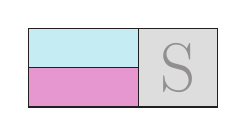
\begin{tikzpicture}[base]
    \widefont \Huge
        \draw [black, fill=C] (0,0) rectangle (1 + 0.4, 0.5);
        \draw [black, fill=G] (0,0.5) rectangle (1 + 0.4, 1);
        \draw [black, fill=lightgrey] (1 + 0.4,0) rectangle (2 + 0.4, 1);
        \node [,darkgrey] at (1.5 + 0.4,0.5) {S};
        \path [use as bounding box] (0,0) rectangle (2 + 0.4,1);
    \end{tikzpicture}
}

\newsavebox{\N}
\savebox{\N}{%
    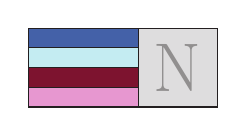
\begin{tikzpicture}[base]
    \widefont \Huge
        \draw [black, fill=C] (0,0) rectangle (1 + 0.4, 0.25);
        \draw [black, fill=U] (0,0.25) rectangle (1 + 0.4, 0.5);
        \draw [black, fill=G] (0,0.5) rectangle (1 + 0.4, 0.75);
        \draw [black, fill=A] (0,0.75) rectangle (1 + 0.4, 1);
        \draw [black, fill=lightgrey] (1 + 0.4,0) rectangle (2 + 0.4, 1);
        \node [,darkgrey] at (1.5 + 0.4,0.5) {N};
        \path [use as bounding box] (0,0) rectangle (2 + 0.4,1);
    \end{tikzpicture}
}


% greyed out versions for the delete action card

\newsavebox{\Agrey}
\savebox{\Agrey}{%
    
\begin{tikzpicture}[base]
    \widefont \Huge
        \draw [black, fill=darkgrey] (0,0) rectangle (1,1);
        \draw [black, fill=black] (1,0) rectangle (2,1);
        \node [,white] at (1.5,0.5) {A};
        \path [use as bounding box] (0,0) rectangle (2,1);
    \end{tikzpicture}
}

\newsavebox{\Tgrey}
\savebox{\Tgrey}{%
    
\begin{tikzpicture}[base]
    \widefont \Huge
        \draw [black, fill=darkgrey] (0,0) rectangle (1,1);
        \draw [black, fill=black] (1,0) rectangle (2,1);
        \node [,white] at (1.5,0.5) {T};
        \path [use as bounding box] (0,0) rectangle (2,1);
    \end{tikzpicture}
}

\newsavebox{\Cgrey}
\savebox{\Cgrey}{%
    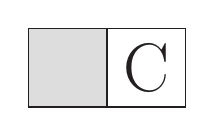
\begin{tikzpicture}[base]
    \widefont \Huge
        \draw [black, fill=lightgrey] (0,0) rectangle (1,1);
        \draw [black, fill=white] (1,0) rectangle (2,1);
        \node [,black] at (1.5,0.5) {C};
        \path [use as bounding box] (0,0) rectangle (2,1);
    \end{tikzpicture}
}

\newsavebox{\Ggrey}
\savebox{\Ggrey}{%
    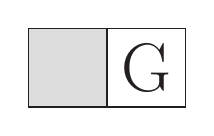
\begin{tikzpicture}[base]
    \widefont \Huge
        \draw [black, fill=lightgrey] (0,0) rectangle (1,1);
        \draw [black, fill=white] (1,0) rectangle (2,1);
        \node [,black] at (1.5,0.5) {G};
        \path [use as bounding box] (0,0) rectangle (2,1);
    \end{tikzpicture}
}


% larger versions for bleed in the corner on nt cards
% 0.4cm trims; TODOv2 make this dynamic

\newsavebox{\Acorner}
\savebox{\Acorner}{%
    
\begin{tikzpicture}[base]
    \widefont \Huge
        \draw [black, fill=A] (0,0) rectangle (1 + 0.4 ,1 + 0.4);
        \draw [black, fill=black] (1 + 0.4,0) rectangle (2 + 0.4,1 + 0.4);
        \node [,white] at (1.5 + 0.4 ,0.5) {A};
        \path [use as bounding box] (0,0) rectangle (2 + 0.4,1 + 0.4);
    \end{tikzpicture}
}

\newsavebox{\Tcorner}
\savebox{\Tcorner}{%
    
\begin{tikzpicture}[base]
    \widefont \Huge
        \draw [black, fill=T] (0,0) rectangle (1 + 0.4,1 + 0.4);
        \draw [black, fill=black] (1 + 0.4,0) rectangle (2 + 0.4,1 + 0.4);
        \node [,white] at (1.5 + 0.4,0.5) {T};
        \path [use as bounding box] (0,0) rectangle (2 + 0.4,1 + 0.4);
    \end{tikzpicture}
}

\newsavebox{\Ccorner}
\savebox{\Ccorner}{%
    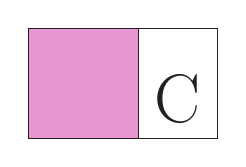
\begin{tikzpicture}[base]
    \widefont \Huge
        \draw [black, fill=C] (0,0) rectangle (1 + 0.4,1 + 0.4);
        \draw [black, fill=white] (1 + 0.4,0) rectangle (2 + 0.4,1 + 0.4);
        \node [,black] at (1.5 + 0.4,0.5) {C};
        \path [use as bounding box] (0,0) rectangle (2 + 0.4,1 + 0.4);
    \end{tikzpicture}
}

\newsavebox{\Gcorner}
\savebox{\Gcorner}{%
    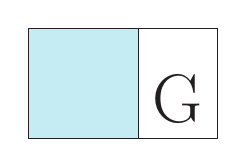
\begin{tikzpicture}[base]
    \widefont \Huge
        \draw [black, fill=G] (0,0) rectangle (1 + 0.4,1 + 0.4);
        \draw [black, fill=white] (1 + 0.4,0) rectangle (2 + 0.4,1 + 0.4);
        \node [,black] at (1.5 + 0.4,0.5) {G};
        \path [use as bounding box] (0,0) rectangle (2 + 0.4,1 + 0.4);
    \end{tikzpicture}
}


% no bleed versions for ac, instructions

\newsavebox{\Anb}
\savebox{\Anb}{%
    
\begin{tikzpicture}[base]
    \widefont \Huge
        \draw [black, fill=A] (0,0) rectangle (1,1);
        \draw [black, fill=black] (1,0) rectangle (2,1);
        \node [,white] at (1.5,0.5) {A};
        \path [use as bounding box] (0,0) rectangle (2,1);
    \end{tikzpicture}
}

\newsavebox{\Tnb}
\savebox{\Tnb}{%
    
\begin{tikzpicture}[base]
    \widefont \Huge
        \draw [black, fill=T] (0,0) rectangle (1,1);
        \draw [black, fill=black] (1,0) rectangle (2,1);
        \node [,white] at (1.5,0.5) {T};
        \path [use as bounding box] (0,0) rectangle (2,1);
    \end{tikzpicture}
}

\newsavebox{\Unb}
\savebox{\Unb}{%
    
\begin{tikzpicture}[base]
    \widefont \Huge
        \draw [black, fill=U] (0,0) rectangle (1,1);
        \draw [black, fill=black] (1,0) rectangle (2,1);
        \node [,white] at (1.5,0.5) {U};
        \path [use as bounding box] (0,0) rectangle (2,1);
    \end{tikzpicture}
}

\newsavebox{\Cnb}
\savebox{\Cnb}{%
    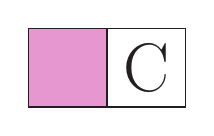
\begin{tikzpicture}[base]
    \widefont \Huge
        \draw [black, fill=C] (0,0) rectangle (1,1);
        \draw [black, fill=white] (1,0) rectangle (2,1);
        \node [,black] at (1.5,0.5) {C};
        \path [use as bounding box] (0,0) rectangle (2,1);
    \end{tikzpicture}
}

\newsavebox{\Gnb}
\savebox{\Gnb}{%
    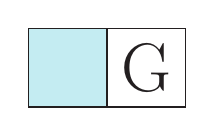
\begin{tikzpicture}[base]
    \widefont \Huge
        \draw [black, fill=G] (0,0) rectangle (1,1);
        \draw [black, fill=white] (1,0) rectangle (2,1);
        \node [,black] at (1.5,0.5) {G};
        \path [use as bounding box] (0,0) rectangle (2,1);
    \end{tikzpicture}
}

\newsavebox{\Rnb}
\savebox{\Rnb}{%
    
\begin{tikzpicture}[base]
    \widefont \Huge
        \draw [black, fill=G] (0,0) rectangle (1, 0.5);
        \draw [black, fill=A] (0,0.5) rectangle (1, 1);
        \draw [black, fill=lightgrey] (1,0) rectangle (2, 1);
        \node [,darkgrey] at (1.5,0.5) {R};
        \path [use as bounding box] (0,0) rectangle (2,1);
    \end{tikzpicture}
}

\newsavebox{\Ynb}
\savebox{\Ynb}{%
    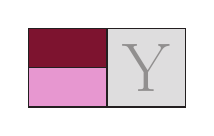
\begin{tikzpicture}[base]
    \widefont \Huge
        \draw [black, fill=C] (0,0) rectangle (1, 0.5);
        \draw [black, fill=U] (0,0.5) rectangle (1, 1);
        \draw [black, fill=lightgrey] (1,0) rectangle (2, 1);
        \node [,darkgrey] at (1.5,0.5) {Y};
        \path [use as bounding box] (0,0) rectangle (2,1);
    \end{tikzpicture}
}

\newsavebox{\HHnb}
\savebox{\HHnb}{%
    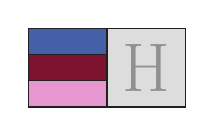
\begin{tikzpicture}[base]
    \widefont \Huge
        \draw [black, fill=C] (0,0) rectangle (1, 0.3333);
        \draw [black, fill=U] (0,0.3333) rectangle (1, 0.6666);
        \draw [black, fill=A] (0,0.6666) rectangle (1, 1);
        \draw [black, fill=lightgrey] (1,0) rectangle (2, 1);
        \node [,darkgrey] at (1.5,0.5) {H};
        \path [use as bounding box] (0,0) rectangle (2,1);
    \end{tikzpicture}
}

\newsavebox{\Bnb}
\savebox{\Bnb}{%
    
\begin{tikzpicture}[base]
    \widefont \Huge
        \draw [black, fill=C] (0,0) rectangle (1, 0.3333);
        \draw [black, fill=U] (0,0.3333) rectangle (1, 0.6666);
        \draw [black, fill=G] (0,0.6666) rectangle (1, 1);
        \draw [black, fill=lightgrey] (1,0) rectangle (2, 1);
        \node [,darkgrey] at (1.5,0.5) {B};
        \path [use as bounding box] (0,0) rectangle (2,1);
    \end{tikzpicture}
}

\newsavebox{\Vnb}
\savebox{\Vnb}{%
    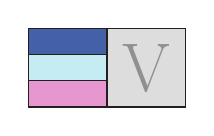
\begin{tikzpicture}[base]
    \widefont \Huge
        \draw [black, fill=C] (0,0) rectangle (1, 0.3333);
        \draw [black, fill=G] (0,0.3333) rectangle (1, 0.6666);
        \draw [black, fill=A] (0,0.6666) rectangle (1, 1);
        \draw [black, fill=lightgrey] (1,0) rectangle (2, 1);
        \node [,darkgrey] at (1.5,0.5) {V};
        \path [use as bounding box] (0,0) rectangle (2,1);
    \end{tikzpicture}
}

\newsavebox{\Dnb}
\savebox{\Dnb}{
    
\begin{tikzpicture}[base]
    \widefont \Huge
        \draw [black, fill=G] (0,0) rectangle (1, 0.3333);
        \draw [black, fill=U] (0,0.3333) rectangle (1, 0.6666);
        \draw [black, fill=A] (0,0.6666) rectangle (1, 1);
        \draw [black, fill=lightgrey] (1,0) rectangle (2, 1);
        \node [,darkgrey] at (1.5,0.5) {D};
        \path [use as bounding box] (0,0) rectangle (2,1);
    \end{tikzpicture}
}

\newsavebox{\Wnb}
\savebox{\Wnb}{%
    
\begin{tikzpicture}[base]
    \widefont \Huge
        \draw [black, fill=U] (0,0) rectangle (1, 0.5);
        \draw [black, fill=A] (0,0.5) rectangle (1, 1);
        \draw [black, fill=lightgrey] (1,0) rectangle (2, 1);
        \node [,darkgrey] at (1.5,0.5) {W};
        \path [use as bounding box] (0,0) rectangle (2,1);
    \end{tikzpicture}
}

\newsavebox{\SSSnb}
\savebox{\SSSnb}{%
    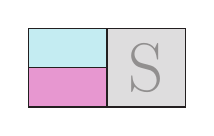
\begin{tikzpicture}[base]
    \widefont \Huge
        \draw [black, fill=C] (0,0) rectangle (1, 0.5);
        \draw [black, fill=G] (0,0.5) rectangle (1, 1);
        \draw [black, fill=lightgrey] (1,0) rectangle (2, 1);
        \node [,darkgrey] at (1.5,0.5) {S};
        \path [use as bounding box] (0,0) rectangle (2,1);
    \end{tikzpicture}
}

\newsavebox{\Nnb}
\savebox{\Nnb}{%
    
\begin{tikzpicture}[base]
    \widefont \Huge
        \draw [black, fill=C] (0,0) rectangle (1, 0.25);
        \draw [black, fill=U] (0,0.25) rectangle (1, 0.5);
        \draw [black, fill=G] (0,0.5) rectangle (1, 0.75);
        \draw [black, fill=A] (0,0.75) rectangle (1, 1);
        \draw [black, fill=lightgrey] (1,0) rectangle (2, 1);
        \node [,darkgrey] at (1.5,0.5) {N};
        \path [use as bounding box] (0,0) rectangle (2,1);
    \end{tikzpicture}
}


%%%%%%%%%%%%%%%%%%%%%%%%%%%%%%%%%%%%%%%%%%%%%%%%%%%%%%%%%%%%%%%%%%%%%%%%%%%%%%%%
%  Draw the molecules
%%%%%%%%%%%%%%%%%%%%%%%%%%%%%%%%%%%%%%%%%%%%%%%%%%%%%%%%%%%%%%%%%%%%%%%%%%%%%%%%

\usepackage{chemfig}
\renewcommand*\printatom[1]{\ensuremath{\mathsf{#1}}}
\setnodestyle{inner sep=0pt, outer sep=0pt, scale=0.9}
\setbondstyle{cap=round, line width=2pt}
\setdoublesep{5pt}
\setatomsep{25pt}
\setbondoffset{3pt}

\tikzset{
  hbond/.style={dotted,blue}
}

\definesubmol{amino}{ {\textcolor{gray}{H_2}}|{\textcolor{gray} N}-[:-30,,,,gray,] }
\definesubmol{acid}{ -[:30,,,,gray,](=[:90,,,,gray,]{\textcolor{gray}{O}})-[:-30,,,,gray,]{\textcolor{gray}O}|{\textcolor{gray}H} }

\newcommand{\molecule}[1]{
    \LARGE #1
}

% amino acids

\newcommand{\alanine}{
    \chemfig[][scale=1.1]{!{amino}(-[:270])!{acid}}
}
\newcommand{\arginine}{
    \chemfig[][scale=1.05]{!{amino}(-[:270]-[:210]-[:270]-[:210]N=[:270](-[:330]NH_2)(-[:210]H_2N))!{acid}}
}
\newcommand{\asparagine}{
    \chemfig[][scale=1.1]{!{amino}(-[:270]-[:210](-[:270]NH_2)(=[:150]O))!{acid}}
}
\newcommand{\aspartate}{
    \chemfig[][scale=1.1]{!{amino}(-[:270]-[:210](-[:270]OH)(=[:150]O))!{acid}}
}
\newcommand{\cysteine}{
    \chemfig[][scale=1.1]{!{amino}(-[:270]-[:210]HS)!{acid}}
}
\newcommand{\glutamine}{
    \chemfig[][scale=1.1]{!{amino}(-[:270]-[:210]-[:270](=[:330]O)(-[:210]H_2N))!{acid}}
}
\newcommand{\glutamate}{
    \chemfig[][scale=1.1]{!{amino}(-[:270]-[:210]-[:270](=[:330]O)(-[:210]HO))!{acid}}
}
\newcommand{\glycine}{
    \chemfig[][scale=1.1]{!{amino}()!{acid}}
}
\newcommand{\histidine}{
    \chemfig[][scale=1.1]{!{amino}(-[:270]-[:210]*5(=-N=-[,,1,1]NH-[,,1,1]))!{acid}}
}
\newcommand{\isoleucine}{
    \chemfig[][scale=1.1]{!{amino}(-[:270](-[:210]-[:270])(-[:330]))!{acid}}
}
\newcommand{\leucine}{
    \chemfig[][scale=1.1]{!{amino}(-[:270]-[:210](-[:270])(-[:150]))!{acid}}
}
\newcommand{\lysine}{
    \chemfig[][scale=1.1]{!{amino}(-[:270]-[:210]-[:270]-[:210]-[:270]NH_2)!{acid}}
}
\newcommand{\methionine}{
    \chemfig[][scale=1.1]{!{amino}(-[:270]-[:210]-[:270]S-[:210])!{acid}}
}
\newcommand{\phenylalanine}{
    \chemfig[line width=2pt, scale=1.1][scale=1.1]{!{amino}(-[:270]-[:210]**6(------))!{acid}}
}
\newcommand{\proline}{
    \chemfig[][scale=1.1]{([:30](=[:90,,,,gray,]{\textcolor{gray}{O}})(-[:330,,,,gray,]{\textcolor{gray}{O}}|{\textcolor{gray}{H}}))(-[:210,,,,gray,]*5(-[,,,2,gray,]{\textcolor{gray}{H}}|{\textcolor{gray}{N}}-[,,2,]---))}
}
\newcommand{\serine}{
    \chemfig[][scale=1.1]{!{amino}(-[:270]-[:210]HO)!{acid}}
}
\newcommand{\threonine}{
    \chemfig[][scale=1.1]{!{amino}(-[:270](-[:210]HO)(-[:330]))!{acid}}
}
\newcommand{\tryptophan}{
    \chemfig[line width=2pt, scale=1.1][scale=1.1]{!{amino}(-[:270]-[:210]*5(=-HN-**6(------)--))!{acid}}
}
\newcommand{\tyrosine}{
    \chemfig[line width=2pt, scale=1.1][scale=1.1]{!{amino}(-[:270]-[:210]**6(---(-HO)---))!{acid}}
}
\newcommand{\valine}{
    \chemfig[][scale=1.1]{!{amino}(-[:270](-[:210])(-[:330]))!{acid}}
}


% bases

\newcommand{\adenine}{
    %\chemfig[line width=2pt, scale=1.1][scale=1.1]{[:-120]-[,2]*5(-[,,,2]HN-[,,2,]*6(-N=-@{a2}N=(-@{a1}NH_2)-=)--N=-)}  % doesn't work -[,,,2]HN-[,,2,]
    \chemfig[line width=2pt, scale=1.1][scale=1.1]{[:-210]N@{a1}H_2-*6(-*5(-N=(-[,2])-[,,,2]HN-[,,2]-)=-N=-@{a2}N=)}     % exactly the same but works
}

\newcommand{\thymine}{
    %\chemfig[line width=2pt, scale=1.1][scale=1.1]{[:60]-[,2]N*6(-=(-CH_3)-(=@{t1}O)-[,,,2]@{t2}HN-[,,2,](=O)-)}
    \chemfig[line width=2pt, scale=1.1, rotate=180][scale=1.1, rotate=180]{[:-120]-[,2]N*6(-=(-H_3C)-(=@{t1}O)-[,,,1]N@{t2}H-[,,1,](=O)-)}
    %@{t2}HN*6(-(=O)-N(-)-=(-CH_3)-(=@{t1}O)-)}
}

\newcommand{\hbondat}{
    \chemmove{ \draw[lightgray, dashed, shorten >=15pt, shorten <=5pt, line width=2pt, line cap=round] (a1)--(t1); }
    \chemmove{ \draw[lightgray, dashed, shorten >=15pt, shorten <=5pt, line width=2pt, line cap=round] (a2)--(t2); }
}

\newcommand{\guanine}{
    %\chemfig[line width=2pt, scale=1.1][scale=1.1]{[:120]-[,2]N*5(-*6(-N=(-@{g3}NH_2)-[,,,1]@{g2}NH-[,,1,](=@{g1}O)-=)--N=-)}
    \chemfig[line width=2pt, scale=1.1, rotate=180][scale=1.1, rotate=180]{[:-60]-[,2]N*5(-*6(-N=(-@{g3}H_2N)-[,,,2]@{g2}HN-[,,2,](=@{g1}O)-=)--N=-)}
}

\newcommand{\cytosine}{
    \chemfig[line width=2pt, scale=1.1][scale=1.1]{[:-120]-[,2]N*6(-=-(-@{c1}H_2N)=@{c2}N-(=@{c3}O)-)}
}

\newcommand{\hbondgc}{
    \chemmove{ \draw[lightgray, dashed, shorten >=5pt, shorten <=15pt, line width=2pt, line cap=round] (g1)--(c1); }
    \chemmove{ \draw[lightgray, dashed, shorten >=5pt, shorten <=15pt, line width=2pt, line cap=round] (g2)--(c2); }
    \chemmove{ \draw[lightgray, dashed, shorten >=5pt, shorten <=15pt, line width=2pt, line cap=round] (g3)--(c3); }
}


%%%%%%%%%%%%%%%%%%%%%%%%%%%%%%%%%%%%%%%%%%%%%%%%%%%%%%%%%%%%%%%%%%%%%%%%%%%%%%%%%%%
%  Macros for the Amino acid cards
%%%%%%%%%%%%%%%%%%%%%%%%%%%%%%%%%%%%%%%%%%%%%%%%%%%%%%%%%%%%%%%%%%%%%%%%%%%%%%%%

\usetikzlibrary{shapes}

\newcommand{\codon}[3]{%
        \node [anchor=west, yshift=2.5cm] at (stock page.west) {\usebox{#1}};
        \node [anchor=west, yshift=1.5cm] at (stock page.west) {\usebox{#2}};
        \node [anchor=west, yshift=0.5cm] at (stock page.west) {\usebox{#3}};
}

\newcommand{\codons}[6]{%
        \node [anchor=west, yshift=2.5cm] at (stock page.west) {\usebox{#1}};
        \node [anchor=west, yshift=1.5cm] at (stock page.west) {\usebox{#2}};
        \node [anchor=west, yshift=0.5cm] at (stock page.west) {\usebox{#3}};
        \node [anchor=west, yshift=-1cm] at (stock page.west) {\usebox{#4}};
        \node [anchor=west, yshift=-2cm] at (stock page.west) {\usebox{#5}};
        \node [anchor=west, yshift=-3cm] at (stock page.west) {\usebox{#6}};
}

\newcommand{\group}[2]{
    \narrowfont
    \node (first) [anchor = west, xshift=-1cm, yshift=0.5cm] at (trimmed page.south east) {#1};
    \node (firsttext) [anchor=east, left=0.2 of first.west] {\scalefont{1.4}{#2}};
}
\newcommand{\groups}[4]{
    \narrowfont 
    \node (first) [anchor = west, xshift=-1cm, yshift=0.5cm] at (trimmed page.south east) {#1};
    \node (firsttext) [anchor=east, left=0.2 of first.west] {\scalefont{1.4}{#2}};
    \node (second) [anchor = west, xshift=-1cm, yshift=1.25cm] at (trimmed page.south east) {#3};
    \node (secondtext) [anchor=east, left = 0.2 of second.west] {\scalefont{1.4}{#4}};
}

\newcommand{\namealiphatic}{Aliphatic}
\newcommand{\namearomatic}{Aromatic}
\newcommand{\nameunusual}{Unusual}
\newcommand{\nameacidic}{Acidic}
\newcommand{\namebasic}{Basic}
\newcommand{\nameacidderiv}{Acid Deriv.}
\newcommand{\namesmallpolar}{Small Polar}
\newcommand{\namesulfur}{Sulfur}


% TODOv2 maybe merge this: use saveboxes for instructions and commands for cards

\newsavebox{\basicbox}
\savebox{\basicbox}{%
    
\begin{tikzpicture}[base, overlay]
        \draw (0,0) circle (0.17);
        \draw [line width=1pt] (-0.11, 0) -- (0.11,0);
        \draw [line width=1pt] (0, -0.11) -- (0, 0.11);
        \path[use as bounding box] (-0.17, -0.17) rectangle (0.17, 0.17);
    \end{tikzpicture}
}

\newcommand{\basic}{
	
\begin{tikzpicture}[base]
        \draw (0,0) circle (0.17);
        \draw [line width=1pt] (-0.11, 0) -- (0.11,0);
        \draw [line width=1pt] (0, -0.11) -- (0, 0.11);
        \path[use as bounding box] (-0.17, -0.17) rectangle (0.17, 0.17);
    \end{tikzpicture}
}

\newsavebox{\acidicbox}
\savebox{\acidicbox}{%
    
\begin{tikzpicture}[base, overlay]
        \draw (0,0) circle (0.17);
        \draw [line width=1pt] (-0.11, 0) -- (0.11,0);
        \path[use as bounding box] (-0.17, -0.17) rectangle (0.17, 0.17);
    \end{tikzpicture}
}

\newcommand{\acidic}{
	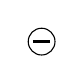
\begin{tikzpicture}[base]
        \draw (0,0) circle (0.17);
        \draw [line width=1pt] (-0.11, 0) -- (0.11,0);
        \path[use as bounding box] (-0.17, -0.17) rectangle (0.17, 0.17);
    \end{tikzpicture}
}


\newsavebox{\aromaticbox}
\savebox{\aromaticbox}{%
    \begin{tikzpicture}[base, overlay]
    \node at (0,0) { \chemfig[scale=0.2, line width=0.5pt][scale=0.2]{**6(-[,,,,,line width=1.0pt]-[,,,,,line width=1.0pt]-[,,,,,line width=1.0pt]-[,,,,,line width=1.0pt]-[,,,,,line width=1.0pt]-[,,,,,line width=1.0pt])}};
    \end{tikzpicture}
}

\newcommand{\aromatic}{
    \chemfig[scale=0.25, line width=0.5pt][scale=0.25]{**6(-[,,,,,line width=1.0pt]-[,,,,,line width=1.0pt]-[,,,,,line width=1.0pt]-[,,,,,line width=1.0pt]-[,,,,,line width=1.0pt]-[,,,,,line width=1.0pt])}
}


\newsavebox{\aliphaticbox}
\savebox{\aliphaticbox}{%
    \begin{tikzpicture}[base, overlay]
    \node at (0,0) { \chemfig[][scale=0.3]{-[:30,,,,,line width=1.0pt]-[:-30,,,,,line width=1.0pt]-[:30,,,,,line width=1.0pt]} };
    \end{tikzpicture}
}

\newcommand{\aliphatic}{
    %\chemfig[][scale=0.3]{-[:30,,,,,line width=1pt]-[:-30,,,,,line width=1pt]-[:30,,,,,line width=1pt]-[:-30,,,,,line width=1pt]-[:30,,,,,line width=1pt]}
    \chemfig[][scale=0.3]{-[:30,,,,,line width=1.0pt]-[:-30,,,,,line width=1.0pt]-[:30,,,,,line width=1.0pt]}
}


\newsavebox{\sulfurbox}
\savebox{\sulfurbox}{%
    
\begin{tikzpicture}[base, overlay]
        \narrowfont
        \scalefont{.8}{} \selectfont
        \node [draw, regular polygon,regular polygon sides=6, minimum size=.3] at (0,0) {S};
    \end{tikzpicture}
}

\newcommand{\sulfur}{
	
\begin{tikzpicture}[base]
        \node [draw, regular polygon,regular polygon sides=6, minimum size=.3] at (0,0) {S};
        %\path[use as bounding box] (-0.15, -0.15) rectangle (0.15, 0.15);
    \end{tikzpicture}
}


\newsavebox{\acidderivbox}
\savebox{\acidderivbox}{%
    
\begin{tikzpicture}[base, overlay]
        \narrowfont
        \scalefont{.8}{} \selectfont
        \node [draw, regular polygon,regular polygon sides=7, minimum size=.3] at (0,0) {N};
    \end{tikzpicture}
}

\newcommand{\acidderiv}{
	
\begin{tikzpicture}[base]
        \node [draw, regular polygon,regular polygon sides=7, minimum size=.3] at (0,0) {N};
        %\path[use as bounding box] (-0.15, -0.15) rectangle (0.15, 0.15);
    \end{tikzpicture}
}


\newsavebox{\smallpolarbox}
\savebox{\smallpolarbox}{%
    
\begin{tikzpicture}[base, overlay]
        \draw [line width=1pt] (-0.15,-0.15) -- (0.15,-0.15) arc (-90:90:0.15) -- (-0.15,0.15) arc (90:270:0.15);
        \draw (-0.24, 0) -- (-0.06,0);
        \draw (-0.15, -0.09) -- (-0.15, 0.09);
        \draw (0.06, 0) -- (0.24,0);
    \end{tikzpicture}
}

\newcommand{\smallpolar}{
	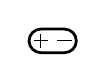
\begin{tikzpicture}[base]
        \draw [line width=1pt] (0,-0.15) -- (0.30,-0.15) arc (-90:90:0.15) -- (0,0.15) arc (90:270:0.15);
        \draw (-0.09, 0) -- (0.09,0);
        \draw (0, -0.09) -- (0, 0.09);
        \draw (0.21, 0) -- (0.39,0);
        %\path[use as bounding box] (-0.15, -0.15) rectangle (0.6, 0.15);
    \end{tikzpicture}
}

\newsavebox{\unusualbox}
\savebox{\unusualbox}{%
    
\begin{tikzpicture}[base, overlay]
        \draw (0,0) circle (0.15);
        \draw (0,0) circle (0.05);
        \draw (0,0.1) circle (0.05);
        \draw (0.1,0) circle (0.05);
        \draw (-0.1,0) circle (0.05);
        \draw (0,-0.1) circle (0.05);
        \draw (-0.18, 0) -- (0.18,0);
        \draw (0, -0.18) -- (0, 0.18);
        \path[use as bounding box] (-0.17, -0.17) rectangle (0.17, 0.17);
    \end{tikzpicture}
}



\newcommand{\unusual}{
	
\begin{tikzpicture}[base]
        \draw (0,0) circle (0.15);
        \draw (0,0) circle (0.05);
        \draw (0,0.1) circle (0.05);
        \draw (0.1,0) circle (0.05);
        \draw (-0.1,0) circle (0.05);
        \draw (0,-0.1) circle (0.05);
        \draw (-0.18, 0) -- (0.18,0);
        \draw (0, -0.18) -- (0, 0.18);
        \path[use as bounding box] (-0.17, -0.17) rectangle (0.17, 0.17);
    \end{tikzpicture}
}

\newsavebox{\hydro}
\savebox{\hydro}{%
    \begin{tikzpicture}[base]
        % counterclockwise: bottom, farthest right, top point, farthest left, bottom
        \draw [fill=lightblue] (0,0) to[out=0,in=-90] (0.18,0.21) to[out=90,in=250] (0.014,0.6) to [out=215, in=90] (-0.225,0.225) to [out=270, in=180] (0,0);
        \path[use as bounding box] (-0.15, 0) rectangle (0.12, 0.4);
    \end{tikzpicture}
}

\newsavebox{\hydrotiny}
\savebox{\hydrotiny}{%
    \begin{tikzpicture}[base, overlay]
        % counterclockwise: bottom, farthest right, top point, farthest left, bottom
        %\draw [fill=lightblue] (0,0) to[out=0,in=-90] (0.12,0.14) to[out=90,in=250] (0.01,0.4) to [out=215, in=90] (-0.15,0.15) to [out=270, in=180] (0,0);
        %\draw [fill=lightblue] (0,0) to[out=0,in=-90] (0.06,0.07) to[out=90,in=250] (0.005,0.2) to [out=215, in=90] (-0.075,0.0715) to [out=270, in=180] (0,0);
        \draw [fill=lightblue] (0,0) to[out=0,in=-90] (0.09,0.105) to[out=90,in=250] (0.0075,0.3) to [out=215, in=90] (-0.1125,0.1125) to [out=270, in=180] (0,0);
        \path[use as bounding box] (0, 0) rectangle (-0.1, 0.1);
    \end{tikzpicture}
}

\newsavebox{\hydrobig}
\savebox{\hydrobig}{%
    \begin{tikzpicture}[base]
        % counterclockwise: bottom, farthest right, top point, farthest left, bottom
        \draw [thick, fill=lightblue] (0,0) to[out=0,in=-90] (0.48,0.56) to[out=90,in=250] (0.04,1.6) to [out=215, in=90] (-0.6,0.6) to [out=270, in=180] (0,0);
        \path[use as bounding box] (-0.6, 0) rectangle (0.48, 1.6);
    \end{tikzpicture}
}

\newsavebox{\hydrobigwhite}
\savebox{\hydrobigwhite}{%
    \begin{tikzpicture}[base]
        % counterclockwise: bottom, farthest right, top point, farthest left, bottom
        \draw [thick, fill=white] (0,0) to[out=0,in=-90] (0.48,0.56) to[out=90,in=250] (0.04,1.6) to [out=215, in=90] (-0.6,0.6) to [out=270, in=180] (0,0);
        \path[use as bounding box] (-0.6, 0) rectangle (0.48, 1.6);
    \end{tikzpicture}
}

%%%%%%%%%%%%%%%%%%%%%%%%%%%%%%%%%%%%%%%%%%%%%%%%%%%%%%%%%%%%%%%%%%%%%%%%%%%%%
%  Amino acid card
%%%%%%%%%%%%%%%%%%%%%%%%%%%%%%%%%%%%%%%%%%%%%%%%%%%%%%%%%%%%%%%%%%%%%%%%%%%%%%%%
\usetikzlibrary{matrix}



\newcommand{\aacard}[7]{
    \begin{tikzpicture}[card]
       
        % one letter code
        \node[anchor = north west, xshift=0.125cm, yshift=-0.25cm](letter) at (trimmed page.north west) { \widefont\Huge\textcolor{black}{\textbf{\scalefont{2}#1\\}} };

        % three letter code
        \node[right = 0.1cm of letter.north east, anchor = north west, baseline] (threeletter) { \textcolor{black}{#2\\} };

        \ifthenelse{\equal{#7}{hydrophilic}}
           { 
                \node[anchor=south west, right=0.1cm of letter.south east, yshift=0.3cm] {\usebox{\hydro}};
           }
           {}


        % name
        \node[anchor = north east, xshift=-0.25cm, yshift=-0.25cm] (name) at (trimmed page.north east) { \narrowfont\Huge\sffamily #3 };


        % codon(s)
        #4;

        % molecule
        \ifthenelse{\equal{#1}{Y}}
        {
            \node[xshift = 0.3cm] at (trimmed page.center) {#5};
        }
        {
            \node[xshift = 1cm] at (trimmed page.center) {#5};
        }

        % group(s) 
        #6;

    \end{tikzpicture}
    \clearpage
}


\newcommand{\sq}[1]{
\draw[fill=#1, draw=none] (0,0) rectangle (\textwidth * 0.083333, \textheight * 0.0625); 
}

\newcommand{\sqt}[1]{
\draw[fill=#1, draw=none] (0,0) rectangle (\textwidth * 0.083333, \textheight * 0.0625 + \trimtop); 
}

\newcommand{\sqe}[1]{
\draw[fill=#1, draw=none] (0,0) rectangle (\textwidth * 0.083333 + \trimedge, \textheight * 0.0625); 
}

\newcommand{\sqc}[1]{
\draw[fill=#1, draw=none] (0,0) rectangle (\textwidth * 0.083333 + \trimedge, \textheight * 0.0625 + \trimtop); 
}

\newcommand{\sqq}[1]{
\draw[fill=#1, draw=none] (0,0) rectangle (\textwidth * 0.5 + \trimedge, \textheight * 0.5 + \trimtop); 
}

\newcommand{\aaback} {
}


%%%%%%%%%%%%%%%%%%%%%%%%%%%%%%%%%%%%%%%%%%%%%%%%%%%%%%%%%%%%%%%%%%%%%%%%%%%%%%%%
%  Nucleotide card
%%%%%%%%%%%%%%%%%%%%%%%%%%%%%%%%%%%%%%%%%%%%%%%%%%%%%%%%%%%%%%%%%%%%%%%%%%%%%%%%

\newcommand{\ntcard}[2] {
    \begin{tikzpicture}[card]
        \node[anchor=north west] at (stock page.north west) {\usebox{#1}};
        \node[anchor=north west, rotate = 180] at (stock page.south east) {\usebox{#2}};

        \ifthenelse{\equal{#1}{\Acorner}}
        {
            \node[anchor=north] at (stock page.north) {\molecule{\adenine}};
            \node[anchor=south] at (stock page.south) {\molecule{\thymine}};
            \hbondat;
        }
        {
            \node[anchor=north] at (stock page.north) {\molecule{\cytosine}};
            \node[anchor=south] at (stock page.south) {\molecule{\guanine}};
            \hbondgc;
        }

    \end{tikzpicture}    
    \clearpage
}


%%%%%%%%%%%%%%%%%%%%%%%%%%%%%%%%%%%%%%%%%%%%%%%%%%%%%%%%%%%%%%%%%%%%%%%%%%%%%%%%
%  Game accessory cards
%%%%%%%%%%%%%%%%%%%%%%%%%%%%%%%%%%%%%%%%%%%%%%%%%%%%%%%%%%%%%%%%%%%%%%%%%%%%%%%%

\newcommand{\watercardon} {
}

\newcommand{\watercardoff} {
}

\newcommand{\fiveprime} {
    \begin{tikzpicture}[card]
        \node [yshift=-1cm,xshift=0.5cm](arrowtail) at (trimmed page.north west) [] { };
        \node [yshift=-1cm,xshift=-0.5cm](arrowhead) at (trimmed page.north east) [] { };
        \node[yshift=-0.5cm](five) at (trimmed page.center) {\fontsize{200}{200} \selectfont 5'};
        \draw[-latex, line width=12pt] (arrowtail) -- (arrowhead);

        %\node [yshift=0.5cm,xshift=-0.7cm](littletail) at (trimmed page.south east) [] { };
        %\node [yshift=0.51cm,xshift=-1.5cm](littlehead) at (trimmed page.south east) [] { };
        %\draw[-latex, line width=1pt, color=grey] (littletail) -- (littlehead);
        %\node[text=grey, rotate=180, xshift=1cm, yshift=-1cm] at (trimmed page.south east) {\fontsize{20}{20} \selectfont 3'};
    \end{tikzpicture}
    \clearpage
}

\newcommand{\threeprime} {
    \begin{tikzpicture}[card]
        \node [xshift=0cm,yshift=1cm,xshift=0.5cm](arrowtail) at (trimmed page.south west) [] { };
        \node [xshift=0cm,yshift=1cm,xshift=-0.5cm](arrowhead) at (trimmed page.south east) [] { };

        \node[yshift=0.5cm, text=grey, rotate=180](five) at (trimmed page.center) {\fontsize{200}{200} \selectfont 3'};
        \draw[latex-, line width=12pt, color=grey] (arrowtail) -- (arrowhead);

        \node [yshift=-0.5cm,xshift=0.7cm](littletail) at (trimmed page.north west) [] { };
        \node [yshift=-0.51cm,xshift=1.5cm](littlehead) at (trimmed page.north west) [] { };
        \draw[-latex, line width=1pt, color=black] (littletail) -- (littlehead);
        \node[text=black, xshift=1cm, yshift=-1cm] at (trimmed page.north west) {\fontsize{20}{20} \selectfont 5'};
    \end{tikzpicture}
    \clearpage
}

\newcommand{\referencent} {
    \begin{tikzpicture}[card]
        \node at (trimmed page.center) {placeholder reference nt};
    \end{tikzpicture}    
    \clearpage
}

\newcommand{\referencemutation} {
    \begin{tikzpicture}[card]
        \node at (trimmed page.center) {placeholder reference mut};
    \end{tikzpicture}    
    \clearpage
}

\newcommand{\referencegroups} {
    \begin{tikzpicture}[card]
        \node (AL) at (1,-1)     {\aliphatic{}};
        \node [below=of AL, node distance=0.5cm] (AR) {\aromatic{}};
        \node [below=of AR] (SP) {\smallpolar{}};
        \node [below=of SP] (BA) {\basic{}};
        \node [below=of BA] (AC) {\acidic{}};
        \node [below=of AC] (AD) {\acidderiv{}};
        \node [below=of AD] (SU) {\sulfur{}};
        \node [below=of SU] (UN) {\unusual{}};
    \end{tikzpicture}    
    \clearpage
}

\newcommand{\turnsummaryfront} {
    \begin{tikzpicture}[card]
        \node at (trimmed page.center) {placeholder turn summary front};
    \end{tikzpicture}    
    \clearpage
}

\newcommand{\turnsummaryback} {
    \begin{tikzpicture}[card]
        \node at (trimmed page.center) {placeholder turn summary back};
    \end{tikzpicture}    
    \clearpage
}


%%%%%%%%%%%%%%%%%%%%%%%%%%%%%%%%%%%%%%%%%%%%%%%%%%%%%%%%%%%%%%%%%%%%%%%%%%%%%
%  Action cards
%%%%%%%%%%%%%%%%%%%%%%%%%%%%%%%%%%%%%%%%%%%%%%%%%%%%%%%%%%%%%%%%%%%%%%%%%%%%%%%%

\newcommand{\acback} {
}


\newcommand{\togglewater} {
    \begin{tikzpicture}[card]
        \node[anchor = north west, xshift=0.25cm, yshift=-0.25cm] (action) at (trimmed page.north west) { \narrowfont\Huge\sffamily Toggle Water ON/OFF};
        \node[below = 3cm, text width=5cm] at (trimmed page.center) {Turn the water on or off. };

        \node (leftlevel)   [yshift=-5.0cm]               at (stock page.north west) {};
        \node (firstpeak)   [yshift=-4.6cm, xshift=4.0cm] at (stock page.north west) {};
        \node (firsttrough) [yshift=-4.8cm, xshift=5.0cm] at (stock page.north west) {};
        \node (secondpeak)  [yshift=-4.4cm, xshift=6.5cm] at (stock page.north west) {};
        \node (rightlevel)  [yshift=-5.0cm]               at (stock page.north east) {};
        \draw [fill=lightblue] (stock page.south east) to[out=180,in=0] (stock page.south west) to[out=90,in=270] 
            (leftlevel) to [out=30, in=285] (firstpeak) to [out=315, in=225] (secondpeak) to [out=255, in=315] (rightlevel)
            to [out=270, in=90] (stock page.south east);

        \node[anchor=south east, yshift=0.25cm, xshift=-0.25cm] at (trimmed page.south east) {\usebox{\hydrobigwhite}};

        \node (buypts) [anchor=north east, xshift=-0.25cm, yshift=-0.25cm] at (trimmed page.north east) {Buy: \Huge 0 \normalsize};
        \node (usepts) [below=0.25cm of buypts] {Use: \Huge 1 \normalsize};

    \end{tikzpicture}    
    \clearpage
}

\newcommand{\insertcard} {
    \begin{tikzpicture}[card]
        \node[anchor = north west, xshift=0.25cm, yshift=-0.25cm] (action) at (trimmed page.north west) { \narrowfont\Huge\sffamily Insert };

        \node [below left = 0cm and 0.75cm of trimmed page.center](firstbot) {\usebox{\Tnb}};
        \node [below right = 0cm and 0.75cm of trimmed page.center](secondbot) {\usebox{\Cnb}};
        \node [above = 1.5cm of firstbot] (firsttop)  {\usebox{\Anb}};
        \node [above = 1.5cm of secondbot] (secondtop) {\usebox{\Gnb}};

        \node [below = 3.0cm, text width=3cm, align=center, anchor=center] at (trimmed page.center) {\normalsize Roll the die to insert a random nucleotide anywhere in the sequence.};

        \node (buypts) [anchor=north east, xshift=-0.25cm, yshift=-0.25cm] at (trimmed page.north east) {Buy: \Huge 3 \normalsize};
        \node (usepts) [below=0.25cm of buypts] {Use: \Huge 1 \normalsize};
    \end{tikzpicture}    
    \clearpage
}

\newcommand{\extend} {
    \begin{tikzpicture}[card]
        \node[anchor = north west, xshift=0.25cm, yshift=-0.25cm] (action) at (trimmed page.north west) { \narrowfont\Huge\sffamily Extend };

        \node [below left = 0cm and 0.75cm of trimmed page.center](firstbot) {\usebox{\Tnb}};
        \node [below right = 0cm and 0.75cm of trimmed page.center](secondbot) {\usebox{\Cnb}};
        \node [above = 1.5cm of firstbot] (firsttop)  {\usebox{\Anb}};
        \node [above = 1.5cm of secondbot] (secondtop) {\usebox{\Gnb}};

        \node [below = 3.0cm, text width=3cm, align=center, anchor=center] at (trimmed page.center) {\normalsize Roll the die to insert a random nucleotide at the end of the sequence.};

        \node (buypts) [anchor=north east, xshift=-0.25cm, yshift=-0.25cm] at (trimmed page.north east) {Buy: \Huge 0 \normalsize};
        \node (usepts) [below=0.25cm of buypts] {Use: \Huge 1 \normalsize};
    \end{tikzpicture}    
    \clearpage
}

\newcommand{\delete} {
    \begin{tikzpicture}[card]
        \node[anchor = north west, xshift=0.25cm, yshift=-0.25cm] (action) at (trimmed page.north west) { \narrowfont\Huge\sffamily Delete };

        \node [below left = 0 cm and 0.75cm of trimmed page.center](firstbot) {\usebox{\Tgrey}};
        \node [below right = 0 cm and 0.75cm of trimmed page.center](secondbot) {\usebox{\Cgrey}};
        \node [above = 1.5cm of firstbot] (firsttop)  {\usebox{\Agrey}};
        \node [above = 1.5cm of secondbot] (secondtop) {\usebox{\Ggrey}};

        \node [below = 3.0cm, text width=3cm, align=center, anchor=center] at (trimmed page.center) {\normalsize Delete any nucleotide in the sequence.};

        \node (buypts) [anchor=north east, xshift=-0.25cm, yshift=-0.25cm] at (trimmed page.north east) {Buy: \Huge 2 \normalsize};
        \node (usepts) [below=0.25cm of buypts] {Use: \Huge 1 \normalsize};
    \end{tikzpicture}    
    \clearpage
}

\newcommand{\mutate} {
    \begin{tikzpicture}[card]
        \node[anchor = north west, xshift=0.25cm, yshift=-0.25cm] (action) at (trimmed page.north west) { \narrowfont\Huge\sffamily Mutate };

        \node [below left = 0cm and 0.75cm of trimmed page.center](firstbot) {\usebox{\Tnb}};
        \node [below right = 0cm and 0.75cm of trimmed page.center](secondbot) {\usebox{\Cnb}};
        \node [above = 1.5cm of firstbot] (firsttop)  {\usebox{\Anb}};
        \node [above = 1.5cm of secondbot] (secondtop) {\usebox{\Gnb}};

        \draw[latex-latex, line width=2pt] (firsttop) -- (firstbot);
        \draw[latex-latex, line width=2pt] (secondtop) -- (secondbot);
        \draw[latex-latex, line width=2pt] (firsttop) -- (secondtop);
        \draw[latex-latex, line width=2pt] (firstbot) -- (secondbot);
        \draw[latex-latex, line width=2pt] (firsttop.south east) -- (secondbot.north west);
        \draw[latex-latex, line width=2pt] (secondtop.south west) -- (firstbot.north east);


        \node [below = 3.0cm, text width=3cm, align=center, anchor=center] at (trimmed page.center) {\scalefont{1.4}{Rotate} \normalsize or \scalefont{1.4}{Flip} \\ \selectfont \normalsize any nucleotide \\ in any direction.};

        \node (buypts) [anchor=north east, xshift=-0.25cm, yshift=-0.25cm] at (trimmed page.north east) {Buy: \Huge 5 \normalsize};
        \node (usepts) [below=0.25cm of buypts] {Use: \Huge 3 \normalsize};
    \end{tikzpicture}    
    \clearpage
}

\newcommand{\revcompseq} {
    \begin{tikzpicture}[card]
        \node[anchor = north west, xshift=0.25cm, yshift=-0.25cm] (action) at (trimmed page.north west) { \narrowfont\Huge\sffamily Reverse Complement};

        \node (fiveprime) [above left=1.0cm and 1.5cm of trimmed page.center] {\scalefont{3}{5'}};
        \node (threeprime) [above right=1.0cm and 1.5cm of trimmed page.center, text=grey] {\scalefont{3}{3'}};

        \draw [bend right, line width = 2pt, latex-latex] (fiveprime.south east) to (threeprime.south west);

        \node [below = 2.5cm, text width=3cm, align=center, anchor=center] at (trimmed page.center) {\scalefont{1.4}{Swap} \normalsize the 5' and 3' ends to read the sequence in the opposite direction on the opposite strand.};

        \node (buypts) [anchor=north east, xshift=-0.25cm, yshift=-0.25cm] at (trimmed page.north east) {Buy: \Huge 3 \normalsize};
        \node (usepts) [below=0.25cm of buypts] {Use: \Huge 1 \normalsize};
    \end{tikzpicture}    
    \clearpage
}

\newcommand{\transversion} {
    \begin{tikzpicture}[card]
        \node[anchor = north west, xshift=0.25cm, yshift=-0.25cm] (action) at (trimmed page.north west) { \narrowfont\Huge\sffamily Transversion };

        \node [below left = 0cm and 0.75cm of trimmed page.center](firstbot) {\usebox{\Tnb}};
        \node [below right = 0cm and 0.75cm of trimmed page.center](secondbot) {\usebox{\Cnb}};
        \node [above = 1.5cm of firstbot] (firsttop)  {\usebox{\Anb}};
        \node [above = 1.5cm of secondbot] (secondtop) {\usebox{\Gnb}};

        \draw[latex-latex, line width=2pt] (firsttop.south east) -- (secondbot.north west);
        \draw[latex-latex, line width=2pt] (secondtop.south west) -- (firstbot.north east);

        \node (textblock) [below = 3.0cm, text width=2cm, align=right, anchor=east] at (trimmed page.center) {\scalefont{1.4}{Flip} \\ \selectfont \normalsize any nucleotide \\ vertically.};
        \node (linestart) [right=0.5cm of textblock.north east] {};
        \node (lineend) [right=0.5cm of textblock.south east] {};
        \draw [-latex, line width=2pt] (linestart) -- (lineend);

        \node (buypts) [anchor=north east, xshift=-0.25cm, yshift=-0.25cm] at (trimmed page.north east) {Buy: \Huge 3 \normalsize};
        \node (usepts) [below=0.25cm of buypts] {Use: \Huge 2 \normalsize};
    \end{tikzpicture}    
    \clearpage
}

\newcommand{\transition} {
    \begin{tikzpicture}[card]
        \node[anchor = north west, xshift=0.25cm, yshift=-0.25cm] (action) at (trimmed page.north west) { \narrowfont\Huge\sffamily Transition };

        \node [below left = 0cm and 0.75cm of trimmed page.center](firstbot) {\usebox{\Tnb}};
        \node [below right = 0cm and 0.75cm of trimmed page.center](secondbot) {\usebox{\Cnb}};
        \node [above = 1.5cm of firstbot] (firsttop)  {\usebox{\Anb}};
        \node [above = 1.5cm of secondbot] (secondtop) {\usebox{\Gnb}};

        \draw[latex-latex, line width=2pt] (firsttop) -- (secondtop);
        \draw[latex-latex, line width=2pt] (firstbot) -- (secondbot);

        \node (textblock) [below = 3.0cm, text width=2cm, align=center, anchor=center] at (trimmed page.center) {\scalefont{1.4}{Flip} \\ \selectfont \normalsize any nucleotide \\ horizontally.};
        \node (linestart) [below=0.5cm of textblock.south west] {};
        \node (lineend) [below=0.5cm of textblock.south east] {};
        \draw [-latex, line width=2pt] (linestart) -- (lineend);


        \node (buypts) [anchor=north east, xshift=-0.25cm, yshift=-0.25cm] at (trimmed page.north east) {Buy: \Huge 3 \normalsize};
        \node (usepts) [below=0.25cm of buypts] {Use: \Huge 2 \normalsize};
    \end{tikzpicture}    
    \clearpage
}

\newcommand{\complement} {
    \begin{tikzpicture}[card]
        \node[anchor = north west, xshift=0.25cm, yshift=-0.25cm] (action) at (trimmed page.north west) { \narrowfont\Huge\sffamily Complement };

        \node [below left = 0cm and 0.75cm of trimmed page.center](firstbot) {\usebox{\Tnb}};
        \node [below right = 0cm and 0.75cm of trimmed page.center](secondbot) {\usebox{\Cnb}};
        \node [above = 1.5cm of firstbot] (firsttop)  {\usebox{\Anb}};
        \node [above = 1.5cm of secondbot] (secondtop) {\usebox{\Gnb}};

        \draw [latex-latex, line width=2pt] (firsttop) -- (firstbot);
        \draw [latex-latex, line width=2pt] (secondtop) -- (secondbot);

        \node (arcstart) [below = 3.0cm, text width=3cm, align=center, anchor=center] at (trimmed page.center) {\scalefont{1.4}{Rotate} \\ \selectfont \normalsize any nucleotide \\ 180 degrees.};
        \draw [latex-, line width=2pt] (arcstart) ++(-90:1.25cm) arc (-90:+90:1.25cm);

        \node (buypts) [anchor=north east, xshift=-0.25cm, yshift=-0.25cm] at (trimmed page.north east) {Buy: \Huge 3 \normalsize};
        \node (usepts) [below=0.25cm of buypts] {Use: \Huge 2 \normalsize};
    \end{tikzpicture}    
    \clearpage
}

\newcommand{\compseq} {
    \begin{tikzpicture}[card]
        \node[anchor = north west, xshift=0.25cm, yshift=-0.25cm] (action) at (trimmed page.north west) { \narrowfont\Huge\sffamily Complement Sequence };
        \node[below = 3cm, text width=5cm] at (trimmed page.center) {Rotate every nucleotide in the sequence by 180 degrees. };
    \end{tikzpicture}    
    \clearpage
}

\newcommand{\pcr} {
    \begin{tikzpicture}[card]
        \node[anchor = north west, xshift=0.25cm, yshift=-0.25cm] (action) at (trimmed page.north west) { \narrowfont\Huge\sffamily Polymerase Chain Reaction };
        %picture pcr
        \node[below = 3cm, text width=5cm] at (trimmed page.center) {Extend the nucleotide sequence with copies of itself until you run out of table space. };
        \node (buypts) [anchor=north east, xshift=-0.25cm, yshift=-0.25cm] at (trimmed page.north east) {Buy: \Huge 3 \normalsize};
        \node (usepts) [below=0.25cm of buypts] {Use: \Huge 1 \normalsize};
    \end{tikzpicture}    
    \clearpage
}


